\documentclass[12pt]{article}
\usepackage{newunicodechar}
\usepackage{cite}
\usepackage{braket}
\usepackage{graphicx}
\graphicspath{ {./figures/} }
\newcommand{\hp}{H$_2^+$}
\newcommand{\gr}{$\ket{g}$}

\title{Dissociation dynamics of H$_2^+$ XUV and IR laser fields}
\author{Tobias Becher, Lukas Blecher}
\date{March 2019}

\begin{document}

\maketitle
\begin{abstract}
    
\end{abstract}



\section{H$_2^+$ vibrational eigenstates}
As a first part of the analysis the vibrational eigenstates of \hp in the 
\gr state were calculated. To do so the Hamiltonian was represented on a grid and by using direct diagonalization solved.
The general form of the hamiltonian is given by 
\begin{equation}\label{eqn:generalHamiltonian}
    \hat{H}=\frac{\hat{p}^2}{2\mu}+\hat{V}_{\ket{g}}
\end{equation}
$\mu$ being the reduced mass of the molecule and $V_{\ket{g}}$ the Born-Oppenheimer surface of the \hp electronic ground state.
The (time-independent) Schr\"odinger-equation (SDE) is now solved using a discrete matrix representation in which the Hamiltonian takes the form of

\begin{equation}\label{eqn:discresteHamiltonian}
    \mathbf H=\left({\begin{array}{cccccc}
   V(x_1)+\frac{1}{\Delta x^2} & \frac{-1}{2\Delta x^2} &0& \cdots & &\\
   \frac{-1}{2\Delta x^2} & V(x_2)+\frac{1}{\Delta x^2} & \ddots & & & \\
   0 &\ddots  &\ddots &&&\\
   \vdots&&&&&\\
  \end{array} } \right)
\end{equation}
\begin{figure}
    \centering
    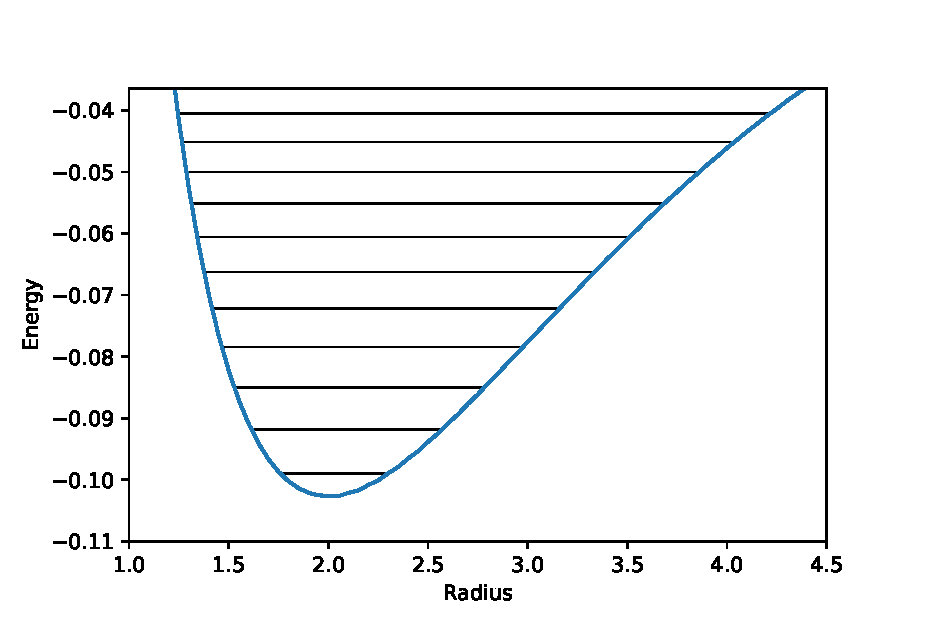
\includegraphics[width=1\textwidth]{vibEigenstates.eps}
    \caption{Vibrational eigenstates of $V_{\ket{g}}$ }
    \label{fig:vib}
\end{figure}
\bibliographystyle{plain}
\bibliography{references}
\end{document}
